\subsection{Aufgabenstellung}

Die Aufgabenstellung ist auf folgender Grafik skizziert. Zentral sind die variablen Bedingungen im Wegenetz. Die Strecke kann durch Pylonen gesperrte Knoten haben. Linien können komplett entfernt sein.  Auf einer Verbindungslinie befindet sich ein Hindernis, welches vom Roboter angehoben werden darf. Der Roboter muss nach dem passieren der Strecke das Hindernis an die ursprüngliche Stelle zurückstellen.  

\begin{figure}[H]
\centering
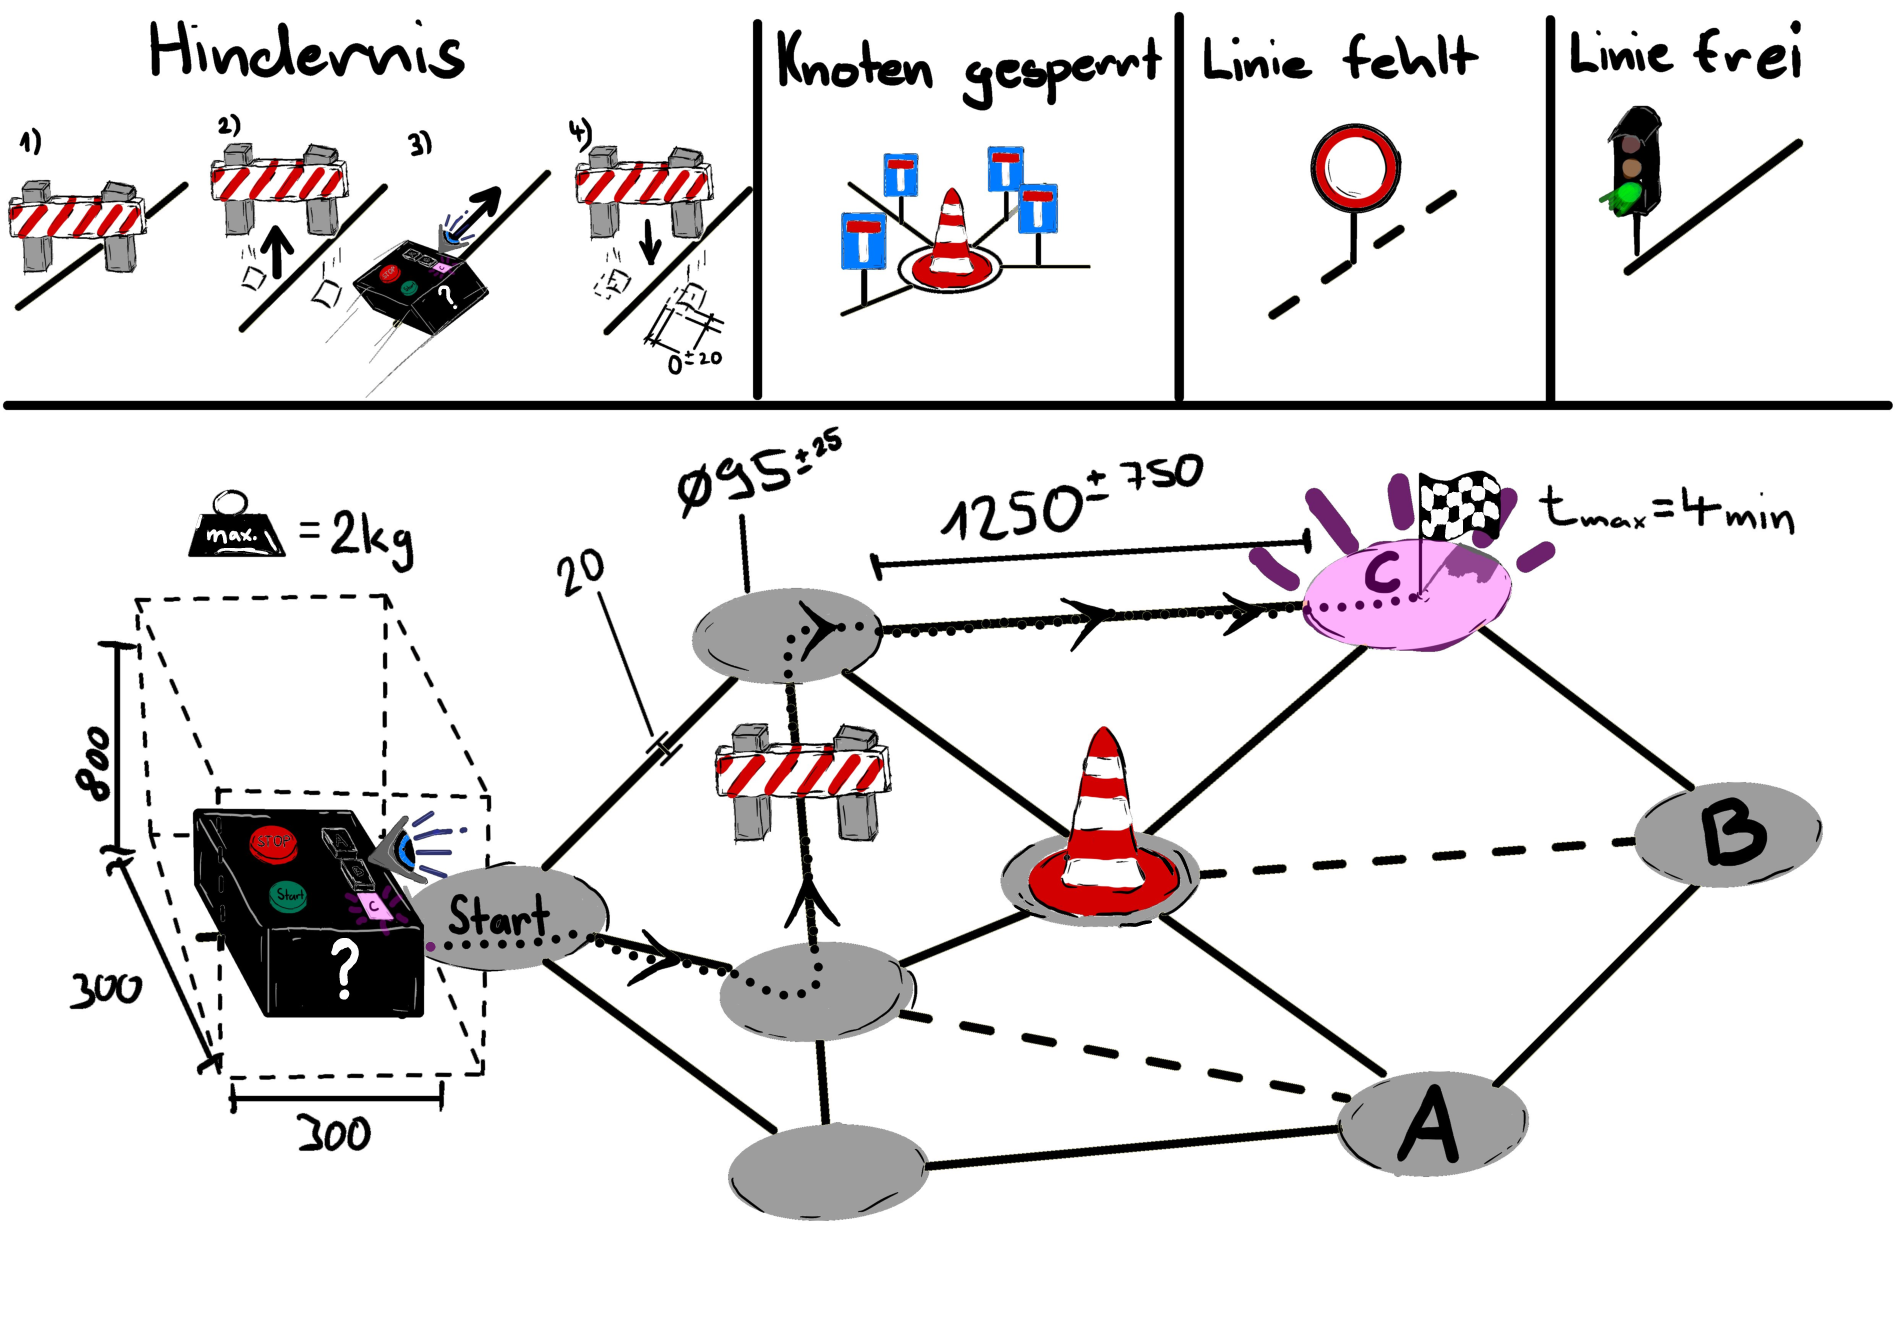
\includegraphics[width=\textwidth]{img/Skizze_Aufgabenstellung_v4.2.png}
\caption{Aufgabenstellung}
\label{fig:aufgebanstellung}
\end{figure}

\subsection{Anforderungsliste}

Die Aufgabenstellung

Die vollständige Anforderungsliste befindet sich im Anhang im Kapitel \nameref{anforderungliste}.